\documentclass[a4paper,14pt]{article}
\usepackage[english, russian]{babel}
\usepackage[utf8]{inputenc}
\usepackage[T2A]{fontenc}

%----------------------------------------------------------------------------------------
%	FONT
%----------------------------------------------------------------------------------------

% % fontspec allows you to use TTF/OTF fonts directly
% \usepackage{fontspec}
% \defaultfontfeatures{Ligatures=TeX}

% % modified for ShareLaTeX use
% \setmainfont[
% SmallCapsFont = Fontin-SmallCaps.otf,
% BoldFont = Fontin-Bold.otf,
% ItalicFont = Fontin-Italic.otf
% ]
% {Fontin.otf}

%----------------------------------------------------------------------------------------
%	PACKAGES
%----------------------------------------------------------------------------------------
\usepackage{url}
\usepackage{parskip} 
\usepackage{csquotes}	

%other packages for formatting
\RequirePackage{color}
\RequirePackage{graphicx}
\usepackage[usenames,dvipsnames]{xcolor}
\usepackage[scale=0.9]{geometry}

%tabularx environment
\usepackage{tabularx}

%for lists within experience section
\usepackage{enumitem}

% centered version of 'X' col. type
\newcolumntype{C}{>{\centering\arraybackslash}X} 

%to prevent spillover of tabular into next pages
\usepackage{supertabular}
\usepackage{tabularx}
\newlength{\fullcollw}
\setlength{\fullcollw}{0.47\textwidth}

%custom \section
\usepackage{titlesec}				
\usepackage{multicol}
\usepackage{multirow}
\usepackage[normalem]{ulem}

%CV Sections inspired by: 
%http://stefano.italians.nl/archives/26
\titleformat{\section}{\Large\scshape\raggedright}{}{0em}{}[\titlerule]
\titlespacing{\section}{0pt}{10pt}{10pt}

%for publications
\usepackage[style=authoryear,sorting=ynt, maxbibnames=2]{biblatex}

%Setup hyperref package, and colours for links
\usepackage[unicode, draft=false]{hyperref}
\definecolor{linkcolour}{rgb}{0,0,0}
\hypersetup{colorlinks,breaklinks,urlcolor=linkcolour,linkcolor=linkcolour}
\addbibresource{citations.bib}
\setlength\bibitemsep{1em}

\usepackage{fontawesome5}
\usepackage{setspace}

\begin{document}

\pagestyle{empty} 
\begin{spacing}{1.5}
    \begin{tabularx}{\linewidth}{@{} C @{}}
        \fbox{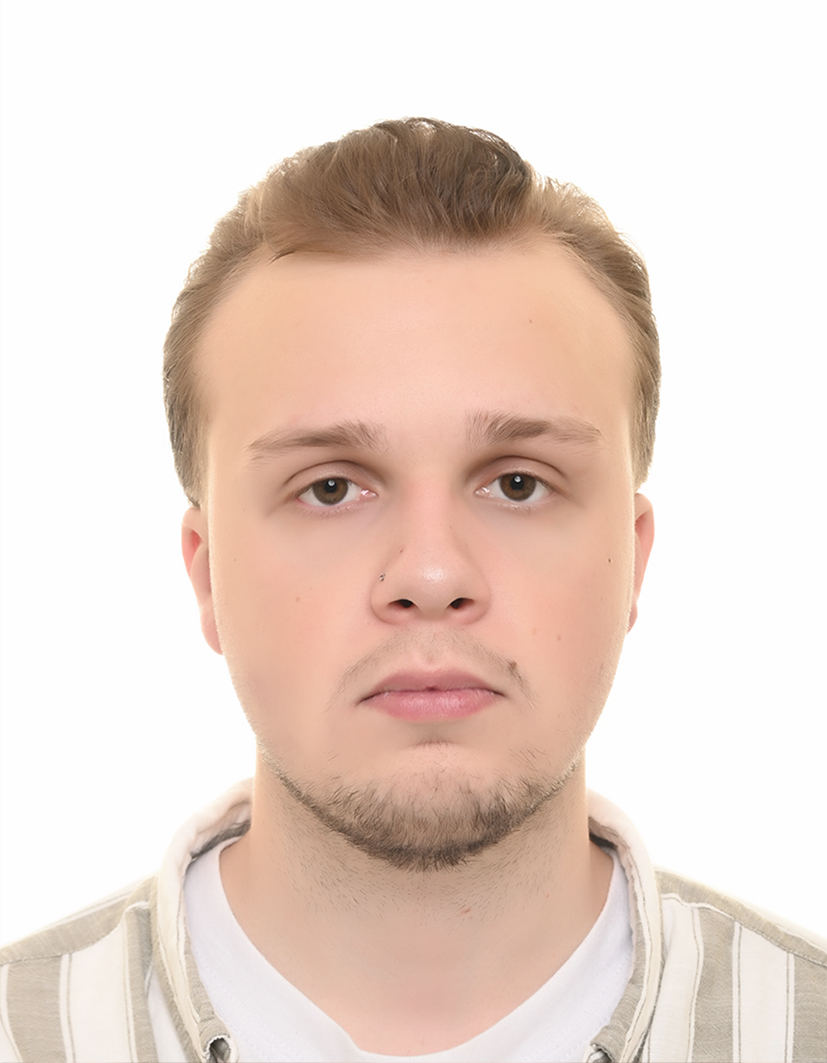
\includegraphics[]{me.jpg}}\\
        \Huge{Артеев Данил} \\[7.5pt]
        \href{https://github.com/arteevdd}{\raisebox{-0.05\height}\faGithub\ arteevdd} \ $|$ \ 
        \href{mailto:arteic4@yandex.ru}{\raisebox{-0.05\height}\faEnvelope \ arteic4@yandex.ru} \ $|$ \ 
        \href{tel:+79195195347}{\raisebox{-0.05\height}\faMobile \ +7-919-519-53-47} \\
    \end{tabularx}
\end{spacing}


\section{\textbf{Опыт работы}}

\begin{tabularx}{\linewidth}{ @{}l r@{} }
    \large\textbf{\href{https://github.com/arteevdd/JavaCourseWork}{\underline{Автоматизация работы библиотеки }}} & \hfill Февраль 2022 - Май 2022 \\[3.75pt]
    \multicolumn{2}{@{}X@{}}{
    \begin{minipage}[t]{\linewidth}
        \begin{itemize}[nosep,after=\strut, leftmargin=2em, itemsep=5pt]
            \large\item Разработал REST API для взаимодействией с базой данных PostgreSQL.
            \large\item Реализовал эндпоинты для взаимодействия извне.
            \large\item Добавил возможность регистрации и авторизации пользователей с помощью Spring Security.
            \large\item Настроил права доступа для пользователей.
        \end{itemize}
        \end{minipage}
    }
    \end{tabularx}



\begin{tabularx}{\linewidth}{ @{}l r@{} }
\large\textbf{Elixir разработчик в компании \href{https://sredasolutions.com/ru}{\underline{Sreda Solutions}}} & \hfill Июль 2022 - Август 2022 \\[3.75pt]
\multicolumn{2}{@{}X@{}}{
\begin{minipage}[t]{\linewidth}
    \begin{itemize}[nosep,after=\strut, leftmargin=2em, itemsep=5pt]
        \large\item Исключил дублирование записей за счёт внедрения дополнительной миграции, тем самым уменьшив количество запросов к базе данных. Новый функционал покрыт тестами.
        \large\item Реализовал получение пути к определённому сервису на стадии \textit{runtime} вместо \textit{compile time}.
        \large\item Разделил функционал создания полиса для корректного возврата средств в случае неудачи. \\ Новый функционал был покрыт тестами.
    \end{itemize}
    \end{minipage}
}
\end{tabularx}

\section{\textbf{Образование}}
\begin{spacing}{1.25}
    \begin{tabularx}{\linewidth}{@{}l X@{}}        
        \large\textbf{Политехнический Университет Петра Великого} & \hfill Август 2020 - Июнь 2024\\
        \large{\textit{Специальность:} Бакалавр, Программная инженерия}           
    \end{tabularx}
    \end{spacing}
    
    \large\textbf{Объектно-ориентированное программирование} $\vert$\textit{ Java} \hfill \normalsize{Сентябрь 2021 - Январь 2022} 
    \begin{itemize}[nosep,after=\strut, leftmargin=2em, itemsep=3pt]
        \item Java Core
        \item Java Concurrency
        \item Collections
        \item Java Multithreading
    \end{itemize}    

    \large{\textbf{Объектно-ориентированное программирование (\textit{Web})} $\vert$\textit{ Java} \hfill \normalsize{ Февраль 2022 - Май 2022}
    \begin{itemize}[nosep,after=\strut, leftmargin=2em, itemsep=3pt]
        \item Написание Backend части для web-приложения с помощью Spring Framework
    \end{itemize}
    
    \large{\textbf{Системное программное обеспечение \textit{GNU/Linux}} $\vert$\textit{ Linux} \hfill \normalsize{Февраль 2021 - Май 2021}
    \begin{itemize}[nosep,after=\strut, leftmargin=2em, itemsep=3pt]
        \item Использование стандартных утилит Linux
    \end{itemize}
    

\section{\textbf{Технические навыки}}
\begin{tabularx}{\linewidth}{@{}l X@{}}
Языки: Java, C++, Elixir\\
Инструменты разработки: Git, VSCode, Clion, Intellij Idea\\
Стэк: Spring Framework, Phoenix Framework, SQL, PostgreSQL, MySQL, MSSQL, Maven, Docker, Flyway, JavaFX, \\Linux


\end{tabularx}

\vfill
% \center{\footnotesize Last updated: \today}

\end{document}
